\chapter{Felhasználói dokumentáció}
\label{ch:user}


\section{Az alkalmazás célja}

Az alkalmazás célja, hogy a felhasználó segítségével membránrendszereket hozzon létre majd szimulálja számításaikat. A membránrendszer egy olyan biológiailag inspirált számítási modell, amely az eukarióta sejtek működését és felépítését követve evolúciós lépéseken keresztül történő információáramlást ír le membránok között. Minden membrán által körbezárt \textit{ún.} régió tartalmaz evolúciós szabályokat, amelyek nem változnak a membránrendszer működése közben. Az információt a rendszerben a régiókban található molekulák, \textit{ún.} objektumok hordozzák. Egy szabály csak akkor tud végbemenni, ha rendelkezésre állnak a szükséges objektumok kellő számban. Ilyen helyzetekben a szabályoknak végre is kell hajtódnia, tehát nem fordulhat elő, hogy minden objektum hozzáférhető, de nem kerül a szabály alkalmazásra. Egy evolúciós lépésben a maximális párhuzamosság elve érvényesül, azaz a szabályok véletszerűen kerülnek kiválasztása, egészen addig, amíg van alkalmazható szabály. Megadhatóak olyan speciális szamályok, amelyek alkalmazásának hatására egy membrán feloldódhat, ilyenkor a tartalma az őt körbevevő régióba kerül. A szabályok között prioritási sorrend is felállítható. A számítás legfontosabb tulajdonsága annak kimenete, amely általában a legkülső régión kívülre (azaz a környezetbe) kijutó objektumok számát jelenti.


\section{Hardver és szoftver követelmények}

A szoftver futtatásához Linux környezetre van szükség, amely támogatja az \verb|ELF| formátumú bináris állományok értelmezését. Ezen felül a futtatási környezetnek rendelkeznie kell \textit{Python interpreterrel}, illetve a \textit{Qt} keretrendszerhez való hozzáférés érdekében \verb|PySide6| modullal. Az utóbbi könnyen megtehető shell környezetben a \verb|pip install PySide6| paranccsal . A program teljes funkcionalitásának kihasználásához a felhasználó számítógépének a bemeneti perifériák közül egérrel és billentyűzettel kell rendelkeznie. A szoftver hardverigénye nem igényel részletesebb specifikációt.


\section{Futtatás}

Mivel a program futtatható állományban kerül a felhasználóhoz, ezért annak az indításhoz elegendő megnyitni a fájlt tartalmazó mappát, majd duplán kattintani a fájlt reprezentáló ikonra. Ugyanez parancssori környezetben is elvégezhető, ilyenkor a terminálban a megfelelő mappába való elnavigálás után a 
\verb|./MembraneSimulator| parancs megadásával futtatható a program.

\section{Grafikus felhasználói felület}

A felhasználó az alkalmazással a grafikus felhasználói felületen keresztül tud kommunikálni, amely a főablakot és az igény szerint megjelenő dialógusablakokat foglalja magába.

\subsection{Főablak}

\begin{figure}[H]
	\centering
	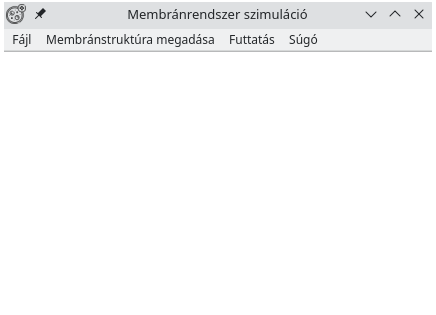
\includegraphics{main_window_empty.png}
	\caption{A főablak az alkalmazás megnyitásakor}
	\label{fig:example-1}
\end{figure}

A főablak az alkalmazás megnyitásakor még tartalmaz egyetlen grafikus elemet sem, viszont a menüsorban található menüpontok segítségével könnyedén változtatni lehet ezen. Ha a felhasználónak nincs korábbi tapasztala a program használatával, akkor érdemes a \textit{Súgó} menüpont kiválasztásával kezdenie, amelyről részletesen szó esik a \ref{help} fejezetben.

\subsection{Dialógusablakok}

A legfontosabb interakció a felhasználó és a szoftver között a dialógisablakokon keresztül történik.  

\subsubsection{Membránstruktúra megadása}

Egy membránrendszer megalkotásának kezdeti módja a struktúrájának megadásával kezdődik. Mivel egy membránrendszerben a membránok hierarchikusan helyezkednek el, ezért a teljes rétegződést nagyon jól lehet ábrázolni fa alakban, ahol mindenkinek a szülő csúcsa az őt legszűkebben tartalmazó régió. Ezzel egyenértékű az a felírás, amikor egyetlen karakterláncban fejezzük ki ugyanezt, azáltal, hogy egy régiót megfeleltetünk egy nyitó-csukó zárójelpárral. Ilyenkor a két zárójel között elhelyezett objektumok jelentik a régió tartalmát. Azonban nem csak objektumok, de más régiók is helyet kaphatnak, ezzel kifejezve azt, hogy a már említett régió közvetlen gyerekét szeretnénk megadni. 

\begin{figure}[H]
	\centering
	\subcaptionbox{Dialógusablak alapmodell létrehozásához}{
		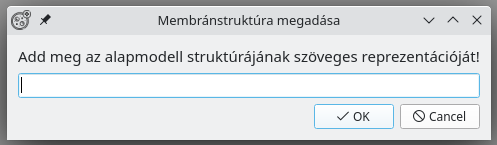
\includegraphics[width=0.45\linewidth]{structure_dialog_base_model.png}}
	\vspace{5pt}
	\subcaptionbox{Dialógusablak szimport-antiport rendszer létrehozásához}{
		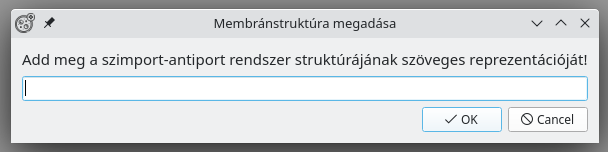
\includegraphics[width=0.45\linewidth]{structure_dialog_symport.png}}
	\caption{Dialógusablakok membránrendszer létrehozásához}
	\label{fig:example-2}
\end{figure}

A \ref{fig:example-2} ábra egy alapmodellbe tartozó membránrendszer struktúrájának megadásahoz használt dialógusablakot mutatja. A megadott karakterláncban a régiók kezdetét és végét jelző zárójelpárok, illetve a bennük előforduló objektumok az angol ábécé kisbetűi szerepelhetnek.

Ha a megadott karakterlánc nem a megfelelő formátumú, akkor a felhasználó figyelmeztetésére egy hibaüzenet jelenik meg a képernyőn. A helyes formátum feltétele, hogy a zárójelpárok karakterein és az szimport-antiport rendszereknél a kimeneti régió jelzésére használt speciális \textit{\#} karakteren kívül csak az angol ábécé kisbetűi szerepelhetnek a bemenetben, illetve annak meg kell felelnie a helyes zárójelezés szabályainak. 



\subsubsection{Objektumok módosítása}
\subsubsection{Szabályok módosítása}
\subsubsection{Szimulációk számának megadása}
\subsubsection{Mentés}
\subsubsection{Betöltés}
\subsubsection{Eredményablak}

\section{Használati útmutató}\label{help}